\section{Project Plan}

We present an idea of what our schedule would be for the project and parts we are imagining.

\subsection{Design of Components}

We envision the best way to build the Passport Tobacco with Nicotine Survey
Data product is to provide a web portal, that provides the user functions to
view many files, search through and download data, and view analytics. 

We would start with a dashboard with some key analytics, and a function bar
with the ability to perform a variety of actions, including search and
analytics.

\begin{figure}[H]
  \centering
  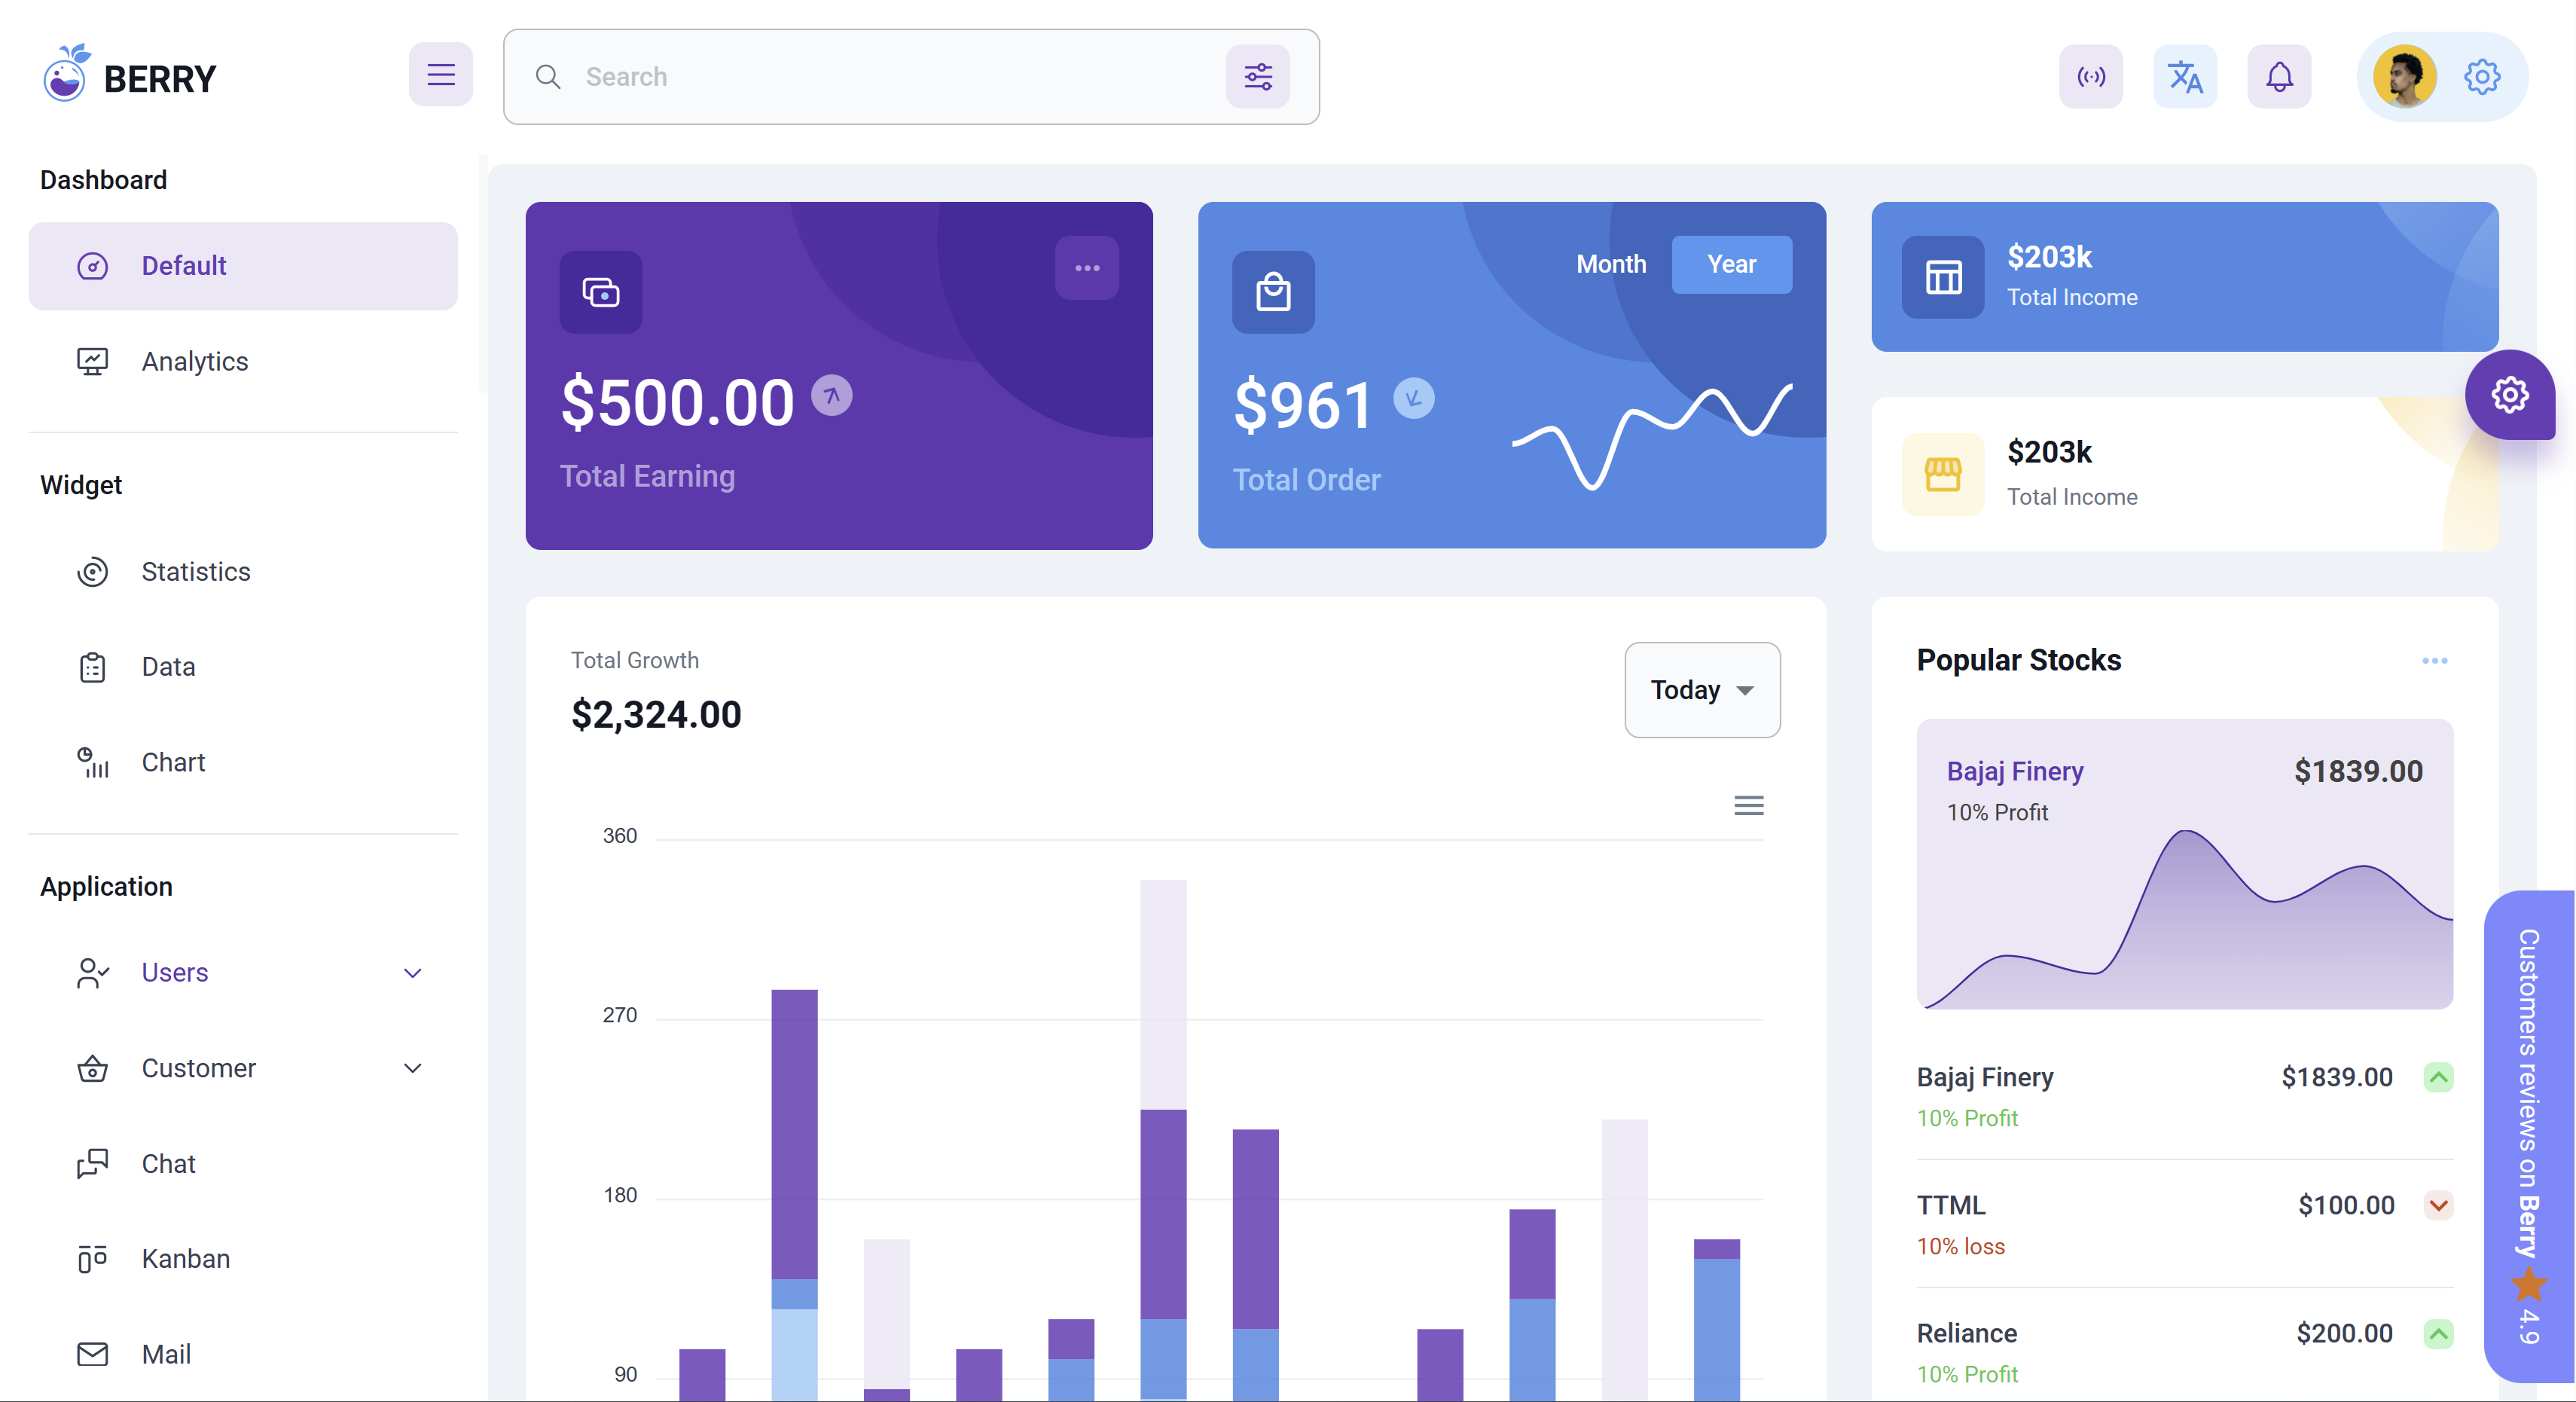
\includegraphics[width=\textwidth]{dashboard.png}
\end{figure}

We would have a high-level design like the diagram below.

\begin{figure}[H]
  \centering
  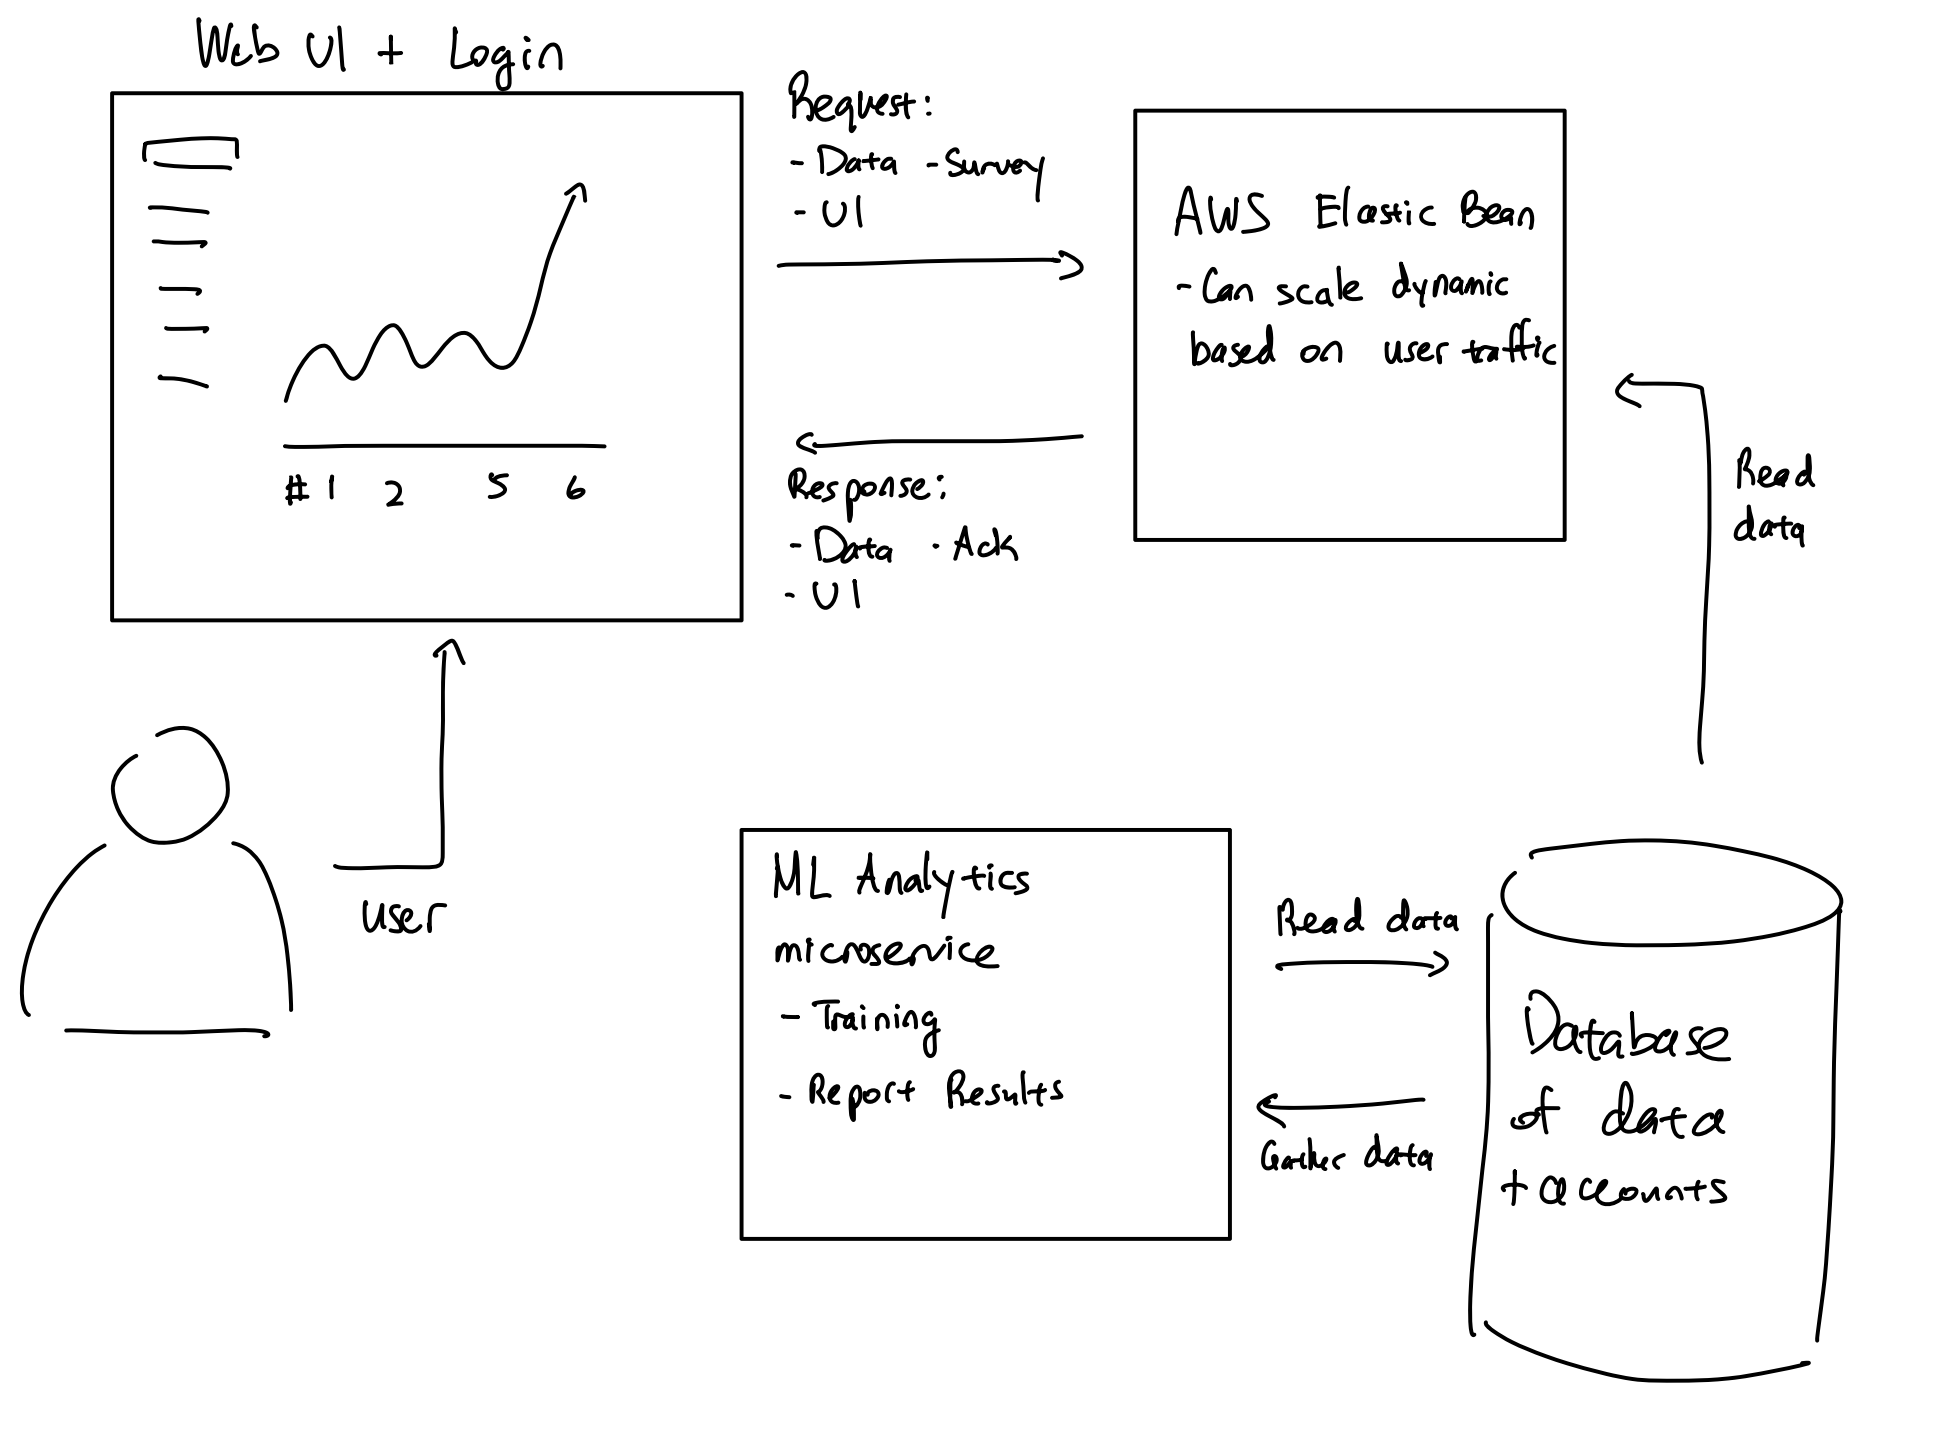
\includegraphics[height=3in]{design.png}
\end{figure}

\subsection{Schedule}

\renewcommand{\arraystretch}{1.3}
\begin{table}[H]
  \centering
  \begin{tabularx}{\textwidth}{|l|X|}
      \hline
      Day 1-5 & Set up web server and login credentials \\\hline
      Month 1 & \begin{minipage}{\linewidth}
        \vspace{6pt}
        \begin{itemize}[itemsep=3pt,parsep=-1pt,leftmargin=*]
        \item Build basic UI for website
        \item Load data into database
        \item Schema design for data
        \end{itemize}
        \vspace{-2pt}
        \end{minipage}\\\hline
      Month 2 & \begin{minipage}{\linewidth}
        \vspace{6pt}
        \begin{itemize}[itemsep=3pt,parsep=-1pt,leftmargin=*]
        \item Build dashboard components to display data: graphs, boxes, legends
        \item Build search API
        \item Add website analytics to track usage
        \end{itemize}
        \vspace{-2pt}
        \end{minipage}\\\hline
      Month 3 & \begin{minipage}{\linewidth}
        \vspace{6pt}
        \begin{itemize}[itemsep=3pt,parsep=-1pt,leftmargin=*]
        \item Build search UI and download ability
        \item Prepare Q1 report
        \end{itemize}
        \vspace{-2pt}
        \end{minipage}\\\hline
      Month 4 & \begin{minipage}{\linewidth}
        \vspace{6pt}
        \begin{itemize}[itemsep=3pt,parsep=-1pt,leftmargin=*]
        \item Build analytics for data
        \item Start training ML models for analytics
        \end{itemize}
        \vspace{-2pt}
        \end{minipage}\\\hline
      Month 5 & \begin{minipage}{\linewidth}
        \vspace{6pt}
        \begin{itemize}[itemsep=3pt,parsep=-1pt,leftmargin=*]
        \item Begin designing survey UI 
        \item Set up schema for survey data collection
        \end{itemize}
        \vspace{-2pt}
        \end{minipage}\\\hline
      Month 6 & \begin{minipage}{\linewidth}
        \vspace{6pt}
        \begin{itemize}[itemsep=3pt,parsep=-1pt,leftmargin=*]
        \item Launch sample survey to test functionality
        \item Prepare for Q2 report
        \end{itemize}
        \vspace{-2pt}
        \end{minipage}\\\hline
      Month 7 & \begin{minipage}{\linewidth}
        \vspace{6pt}
        \begin{itemize}[itemsep=3pt,parsep=-1pt,leftmargin=*]
        \item Build functionality for sharing reports of data
        \item Improve personalized analytics and search
        \item Start a reliability sprint to make sure codebase is good and website is free of bugs
        \end{itemize}
        \vspace{-2pt}
        \end{minipage}\\\hline
      Month 8 & \begin{minipage}{\linewidth}
        \vspace{6pt}
        \begin{itemize}[itemsep=3pt,parsep=-1pt,leftmargin=*]
        \item Build functionality for sharing reports of data (continued)
        \item Begin designing survey UI and data collection
        \end{itemize}
        \vspace{-2pt}
        \end{minipage}\\\hline
      Month 9 & \begin{minipage}{\linewidth}
        \vspace{6pt}
        \begin{itemize}[itemsep=3pt,parsep=-1pt,leftmargin=*]
        \item Address issues with platforms reported by users
        \item Train clients to use our platform
        \item Q3 report
        \end{itemize}
        \vspace{-2pt}
        \end{minipage}\\\hline
      Month 10-12 & \begin{minipage}{\linewidth}
        \vspace{6pt}
        \begin{itemize}[itemsep=3pt,parsep=-1pt,leftmargin=*]
        \item Additional buffer time that will likely be needed to ensure the project finishes on time
        \item Q4 Report and final presentations
        \end{itemize}
        \vspace{-2pt}
        \end{minipage}\\\hline
  \end{tabularx}
\end{table}

\clearpage
\section{Technical Capabilities}

We have expertise a variety of frontend, backend and data tools. Some are
listed below to give an idea, but the list is not exhaustive. Please also see
Section \ref{past_work} to see some of the past work we have taken to see our
work capabilities and quality.

We are able to build systems from scratch, from bare metal, to server racks,
all the way up to design and UI for websites, and including setting up
databases.

\begin{itemize}
  \item \tb{Web technologies}
  \begin{itemize}
    \item React, Angular, Relay, GraphQL
    \item Nodejs, Express, Webpack, Django, Flask
    \item Typescript, SASS
    \item d3.js, AG Grid, Chart.js, three.js
  \end{itemize}
  \item \tb{Machine Learning}
  \begin{itemize}
    \item Neural Networks (GAN, CNN, RNN, Transformers)
    \item PyTorch, Tensorflow, Google Colab
    \item Stable Diffusion, Natural Language Processing, Computer Vision
  \end{itemize}
  \item \tb{Backend and Systems}
  \begin{itemize}
    \item Kubernetes, AWS, Kafka, Redis, Docker
    \item Compilers, Operating systems, embedded systems
  \end{itemize}
  \item \tb{Databases}
  \begin{itemize}
    \item MongoDB, Snowflake, PostgreSQL, MySQL, Oracle, Neo4j
  \end{itemize}
  \item \tb{Security}
  \begin{itemize}
    \item AES, SHA and other industry-standard encryption
    \item User data protection, privacy
  \end{itemize}
  \item \tb{Programming Languages}
  \begin{itemize}
    \item C, C++, C\#, Python, Javascript, PHP, Java, Go, Assembly, System Verilog
  \end{itemize}
\end{itemize}